%! TeX program = luatex
\documentclass{article}
\usepackage{amsmath}
\usepackage{fontspec}
\usepackage[margin=0.75in]{geometry}
\usepackage{tikz}
\usetikzlibrary{arrows}

\setmainfont{Noto Serif CJK KR}
\title{8. 여러 가지 부등식 step C 풀이}
\date{}

\begin{document}
\maketitle
\paragraph{1 (1)번}
원래 부등식은

$$
\begin{cases}
    x^2 - (a + 1)x + a < 0 & \mbox{(a)} \\
    x \ge 3 & \mbox{(b)}
\end{cases}
$$

여기서 (a)를 인수분해하면 $(x - 1)(x - a) < 0$이고, 2가지 경우로 나눌 수 있다.

\subparagraph{1. (a)의 해가 $1 < x < a$인 경우}
부등식을 그림으로 그려보자.

\begin{center}
    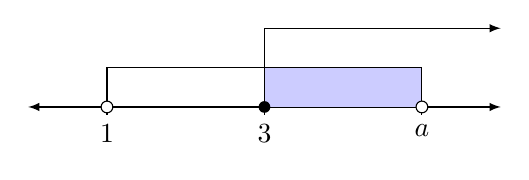
\begin{tikzpicture}
        \draw[latex-latex] (0,0) -- (6,0);
        \fill[blue!20](5,0.5)rectangle(3,0);
        \draw[shift={(1, 0)}, color=black] (0pt,3pt) -- (0pt,-3pt) node[below] {$1$};
        \draw[shift={(3, 0)}, color=black] (0pt,3pt) -- (0pt,-3pt) node[below] {$3$};
        \draw[shift={(5, 0)}, color=black] (0pt,3pt) -- (0pt,-3pt) node[below] {$a$};
        \node[circle,fill,inner sep=1.5pt](a)at(3,0){};
        \node[circle,draw,fill=white,inner sep=1.5pt](b)at(1,0){};
        \node[circle,draw,fill=white,inner sep=1.5pt](c)at(5,0){};
        \draw[-latex,black](a)--++(0,1)--++(3,0);
        \draw[black](b)--(1,0.5)--(5,0.5)--(c);
    \end{tikzpicture}
\end{center}

이 때 부등식의 해가 있으려면 파란색으로 색칠된 부분이 존재해야 한다는 것을 쉽게 알 수 있다. 따라서 이 경우에서는 $a > 3$이 성립하여야 한다.

\subparagraph{2. (a)의 해가 $a < x < 1$인 경우}
방금 전처럼 그림으로 나타내면

\begin{center}
    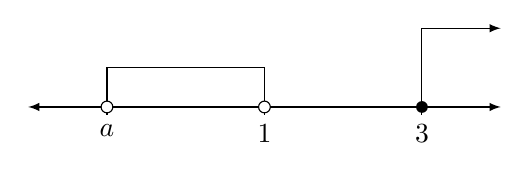
\begin{tikzpicture}
        \draw[latex-latex] (0,0) -- (6,0);
        \draw[shift={(1, 0)}, color=black] (0pt,3pt) -- (0pt,-3pt) node[below] {$a$};
        \draw[shift={(3, 0)}, color=black] (0pt,3pt) -- (0pt,-3pt) node[below] {$1$};
        \draw[shift={(5, 0)}, color=black] (0pt,3pt) -- (0pt,-3pt) node[below] {$3$};
        \node[circle,fill,inner sep=1.5pt](a)at(5,0){};
        \node[circle,draw,fill=white,inner sep=1.5pt](b)at(1,0){};
        \node[circle,draw,fill=white,inner sep=1.5pt](c)at(3,0){};
        \draw[-latex,black](a)--++(0,1)--++(1,0);
        \draw[black](b)--(1,0.5)--(3,0.5)--(c);
    \end{tikzpicture}
\end{center}

그림에서 볼 수 있듯 겹치는 부분이 없으므로 이때 조건을 만족하는 a의 범위는 존재하지 않는다. \newline

따라서 답은 \underline{$a > 3$}이다.

\paragraph{1 (2)번}
원래 부등식은

$$
\begin{cases}
    x^2 + x - 6 > 0 & (a) \\
    \lvert x - a \rvert \le 1 & (b)
\end{cases}
$$

우선 (a)를 인수분해하면 $(x + 3)(x - 2) > 0$이므로 이를 풀면 $x > 2$, $x < -3$이다. 또한, (b)를 풀면 $-1 + a \le x \le 1 + a$임을 알 수 있다. \newline

이 부등식이 해를 가지기 위해서는 $-1 + a < -3$ 또는 $1 + a > 2$이여야 하고, 따라서 이 일차부등식을 풀면 답을 구할 수 있다. \newline

따라서 답은 \underline{$a < -2$, $a > 1$}이다.

\paragraph{2번}

원래 부등식을 다음과 같이 놓자.

$$
\begin{cases}
    x^2 + ax + b < 0 & (a) \\
    x^2 + 3x \ge 0 & (b)
\end{cases}
$$

(b)를 풀면 해가 $x \le -3$, $x \ge 0$임을 알 수 있다. 또한, 주어진 연립부등식의 해가 $0 \le x < 3$인 것을 통해 (a)의 해는 $k < x < 3$의 꼴임을 알 수 있다. 이때 부등식이 성립하는 경우를 그림으로 그려보면 다음과 같다.

\begin{center}
    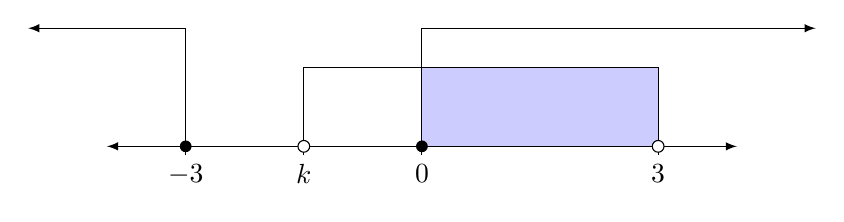
\begin{tikzpicture}
        \draw[latex-latex] (-4,0) -- (4,0);
        \fill[blue!20](0,0)rectangle(3,1);
        \draw[shift={(-3,0)}, color=black] (0pt,3pt) -- (0pt,-3pt) node[below] {$-3$};
        \draw[shift={(-1.5,0)}, color=black] (0pt,3pt) -- (0pt,-3pt) node[below] {$k$};
        \draw[shift={(0,0)}, color=black] (0pt,3pt) -- (0pt,-3pt) node[below] {$0$};
        \draw[shift={(3,0)}, color=black] (0pt,3pt) -- (0pt,-3pt) node[below] {$3$};
        \node[circle,fill,inner sep=1.5pt](a)at(-3,0){};
        \node[circle,fill,inner sep=1.5pt](b)at(0,0){};
        \node[circle,draw,fill=white,inner sep=1.5pt](c)at(-1.5,0){};
        \node[circle,draw,fill=white,inner sep=1.5pt](d)at(3,0){};
        \draw[-latex,black](a)--++(0,1.5)--++(-2,0);
        \draw[-latex,black](b)--++(0,1.5)--++(5,0);
        \draw[black](c)--++(0,1)--++(4.5,0)--++(d);
    \end{tikzpicture}
\end{center}

근과 계수의 관계의 의해 $3 + k = -a$, $3k = b$임을 알 수 있다. $-3 \le k \le 0$이므로 $\lvert a \rvert + \lvert b \rvert = 3 + k - 3k$이고, $3 - 2k = 5$이므로 k는 -1, a는 -2, b는 -3임을 알 수 있고, 이 문제의 답은 \underline{$13$}이 된다.

\paragraph{3번}

주어진 부등식을 정리하면

$$
\lvert (m + 1)(x - 1) \rvert > (m + 1)(m + 2)
$$

이 경우에서 우변의 값의 범위에 따라 몇 가지 경우로 나눌 수 있다.

\subparagraph{1. $(m + 1)(m + 2) < 0$인 경우}
주어진 부등식의 해는 모든 실수이다.

\subparagraph{2a. $m = -1$인 경우}
$0 > 0$이므로 해가 없다. 따라서 $b = -1$이다.

\subparagraph{2b. $m = -2$인 경우}
$\lvert -x + 1 \rvert > 0$이므로 $x \ne 1$이다.

\subparagraph{3. $(m + 1)(m + 2) > 0$인 경우}
절댓값 기호를 풀면

$$
(m + 1)(x - 1) > (m + 1)(m + 2)
$$

또는

$$
(m + 1)(x - 1) < -(m + 1)(m + 2)
$$

임을 쉽게 알 수 있다. \newline

여기서 $m + 1 > 0$이면 $x - 1 > m + 2$ 또는 $x - 1 < -(m + 2)$이고, 이를 풀면 $x > m + 3$ 또는 $x < -(m + 1)$이다. 따라서 $a = 0$이다. \newline

반대로 $m + 1 < 0$이면 $x - 1 < m + 2$ 또는 $x - 1 > -(m + 2)$이고, 이를 방금 전처럼 풀면 $x < m + 3$ 또는 $x > -(m + 1)$이다. 따라서 $c = -2$이다. \newline

정답은 $a = 0$, $b = -1$, $c = -2$이므로 $a - 2b - 3c = \underline{8}$이다.

\paragraph{4번}
주어진 이차방정식을 그래프로 나태냈을 때의 축의 방정식은 $x = -2a$이고, a가 양수이므로 축은 y축 왼쪽에 존재한다는 것을 알 수 있다. 즉, 실근이 존재한다면 적어도 하나는 음수인 것이다. 따라서 주어진 이차방정식이 실근을 가지면 되므로

$$
(4a)^2 - 4(4 - a^2) \ge 0
$$

를 만족하면 되고, 정리하면

$$
20a^2 - 16 \ge 0
$$

이를 풀면 $a \ge \frac{2}{\sqrt{5}}$이고, $m = \frac{2}{\sqrt{5}}$이다. 따라서 답은 $5m^2 = \underline{4}$.

\paragraph{5번}
$t^2 - 2t - 2 = (t - 1)^2 - 3$이고, $f(x)$의 값은 다음과 같이 경우를 나누어 범위를 확인할 수 있다.

\subparagraph{1. $x \le 1 \le x + 2$인 경우}
$x$의 범위는 $-1 \le x \le 1$이고, $f(x) = -3$이므로 정수 $x$로 -1, 0, 1이 가능하다.

\subparagraph{2. $1 < x$인 경우}
$f(x) = x^2 - 2x - 2$이고, $x^2 - 2x - 2 \le x$를 풀면 정수해의 값은 0, 1, 2, 3이다.

\subparagraph{3. $x + 2 < 1$인 경우}
$f(x) = (x + 2)^2 - 2(x + 2) - 2$이고, 이를 정리하면 $f(x) = x^2 + 2x - 2$이다. 이때 $x^2 + 2x - 2 \le x$를 풀면 정수해의 값은 -2, -1, 0, 1이다. \newline

따라서 정수 $x$의 개수는 \underline{6}개이다.

\paragraph{6번}
우선 조건 (가)에 의해 함수 $y = f(x)$의 그래프는 직선 $x = 3$에 의해 대칭임을 알 수 있다. 따라서 문제의 조건을 이용하면 $f(x)$를 다음과 같이 놓을 수 있다.

$$
f(x) = n(x - 3)^2 + m
$$

여기서 $n$, $m$은 자연수이다. (나)를 이용하면 다음 이차방정식은 중근을 갖는다.

$$
n(x - 3)^2 + m = 2x - 4
$$

따라서 판별식을 이용하면 다음과 같다.

$$
(6n + 2)^2 - 4n(9n + m + 4) = 0
$$

이를 간단히 하면

$$
2n - mn + 1 = 0
$$

이고, 이를 통해 $n = 1$, $m = 3$임을 알 수 있다. \newline

$y = f(x)$의 그래프와 직선 $y = kx + 6 + k - k^2$이 서로 다른 두 교점을 가지므로 다음 이차방정식은 서로 다른 두 실근을 가진다.

$$
x^2 - 6x + 12 = kx + 6 + k - k^2
$$

판별식을 이용하여 부등식을 세우고, 정리하면

$$
3k^2 - 16k - 12 < 0
$$

이를 풀면 $-\frac{2}{3} < k < 6$임을 알 수 있다.

따라서 자연수 k로 가능한 것은 1, 2, 3, 4, 5 \underline{6}개임을 알 수 있다.

\end{document}
